\documentclass[problem]{mcs}

\begin{pcomments}
  \pcomment{FP_network_probability}
  \pcomment{from: F08.final}
\end{pcomments}


\pkeywords{
  congestion
  probability
  network
  routing}

%%%%%%%%%%%%%%%%%%%%%%%%%%%%%%%%%%%%%%%%%%%%%%%%%%%%%%%%%%%%%%%%%%%%%
% Problem starts here
%%%%%%%%%%%%%%%%%%%%%%%%%%%%%%%%%%%%%%%%%%%%%%%%%%%%%%%%%%%%%%%%%%%%%

\begin{problem} % \label{network} \ptitle{Packet Racket!}
  The \term{complete ternary-tree network} with 9 inputs and 9 outputs
  is shown below.  When a packet at an input terminal is destined for
  some output terminal, its route is the unique shortest path to the
  designated output terminal.

  Starting with a packet at each input terminal, output destinations
  for the packets will be determined by randomly in two different
  ways.  Let $T$ be the random variable equal to the number of packets
  routed through the dashed edge in the figure.

\vspace{12pt}
\centerline{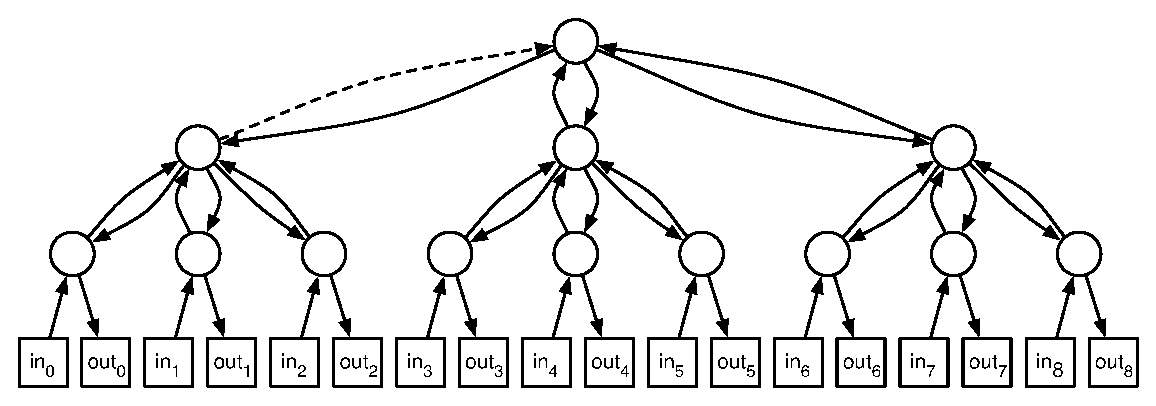
\includegraphics[width=6.5in]{ternary-network}}
\vspace{12pt}

\bparts

% \ppart{??} What is the diameter of this network, including the edges
% connected to the inputs and outputs?
%
% \solution[\vspace{0.5in}]{The diameter is the length of the shortest
%   distance between the input and output that are farthest apart. Any
%   path that goes through the top node is a longest path (for example
%   that from $\mathrm{in_0}$ to $\mathrm{out_8}$) with length 6.}

\ppart\label{I1I12I3} Let $I_0$, $I_1$, and $I_2$ be indicator variables
for the events that a packet originating at $\text{in}_0$, $\text{in}_1$,
and $\text{in}_2$, respectively, gets routed through the dashed edge in
the figure.  Explain why $T=I_0+I_1+I_2$.

\examspace[1in]
\begin{solution}
  The only routes through the dashed edge are ones that originate at
  $\text{in}_0$, $\text{in}_1$, and $\text{in}_2$, so the total number of
  packets routed through the dashed edge will be the same as the total
  number of packets starting from these terminals, namely, $I_0+I_1+I_2$.
\end{solution}

\ppart \label{edgepacketprob} %10
Suppose that the output terminal for each packet is chosen randomly
with a uniform distribution and independently of the other packets.
(Note that outputs may receive packets from multiple inputs including
their corresponding input.)
  \begin{itemize}
  \item What is the probability that the packet at $\text{in}_2$ has one
    of $\text{out}_3$--$\text{out}_8$ as its destination? \hfill\examrule

    \item What is $\expect{T}$? \hfill\examrule
\examspace[0.5in]

    \item What is $\variance{T}$? \hfill\examrule

\end{itemize}
\examspace[0.5in]

\begin{solution}
\begin{align*}
 \pr{\text{$in_2$ is destined for $out_3$--$out_8$}} & = 2/3\\
 \expect{T} & = 2\\
 \variance{T} & = 2/3.
\end{align*}

The packet at input 2 will pass through the dashed edge iff its
destination is one of the six outputs 3--8.  Since the nine outputs
are are chosen as destinations uniformly,
\[
 \pr{\text{$in_2$ is destined for $out_3$--$out_8$}} = 6/9.
\]
But the packet at $\text{in}_2$ gets routed through the dashed edge iff it
is destined for one of $\text{out}_3$--$\text{out}_8$, so $\pr{I_2=1} =
2/3$ and hence $\expect{I_2}=2/3$ and $\variance{I_2} = 2/3(1- 2/3) =
2/9$.  The same reasoning applies to $I_0$ and $I_1$.  By linearity of
expectation,
\[
\expect{T} = \expect{I_0} + \expect{I_1} + \expect{I_2} = 3(2/3) = 2.
\]
Since, the destinations are chosen independently, $I_0$ ,$I_1$ and
$I_2$ are independent, and hence linearity of variance also holds, so
\[
\variance{T} = \variance{I_0} + \variance{I_1} + \variance{I_2} = 3(2/9) = 2/3.
\]

\end{solution}

\ppart\label{uniformpermute} Now suppose input packets are routed to
different output terminals, with all permutations of inputs to outputs
equally likely.  Briefly explain why the expected value of $T$ is the
same as part~\eqref{edgepacketprob}, but the variance may not be.

\examspace[1in]

\begin{solution}
  In this case it is still true that $\pr{I_2 = 1} = 2/3$, and since
  this and linearity of expectation was all that was needed to
  calculate $\expect{T}$ in part~\eqref{edgepacketprob}, the
  expectation in this case is the same.

  However, $I_0,I_1,I_2$ are not pairwise independent.  For example if
  $I_0=1$, then there are only five remaining destinations among
  $\text{out}_3$--$\text{out}_8$, so $\prcond{I_1 = 1}{I_0=1} = 5/9 \neq
  \pr{I_1=1}$.  Now linearity of variance is not guaranteed, and the
  reasoning of part~\eqref{edgepacketprob} no longer applies.
\end{solution}

  \ppart What is $\variance{T}$ when destinations are assigned as in
   part~\eqref{uniformpermute}? \hfill \examrule

\examspace{3in}

\begin{solution}
\begin{align}
\variance{T} & = \expect{T^2} - \expectsq{T}\notag\\
             & = \expect{(I_0+I_1+I_2)^2} - 4
                   & \text{(by parts~\eqref{I1I12I3} and~\eqref{edgepacketprob})}\notag\\
             & = \expect{I_0^2+ I_1^2+ I_2^2+ I_0I_1 +I_0I_2 +I_1I_2}-4\notag\\
             & = 3\expect{(I_0)^2}+ 3\expect{I_0I_1}-4
                  & \text{(by symmetry)}.\label{3eI3eII}
\end{align}
But $I_0^2=I_0$ so $\expect{I_0^2} = 2$, and since $I_0I_1$ is 0-1-valued
\[
\expect{I_0I_1} = \pr{I_0I_1=1}=\prcond{I_1 = 1}{I_0=1}\cdot
\pr{I_0=1} = (5/9)\cdot (2/3) = 10/27.
\]
From~\eqref{3eI3eII}, we conclude
\[
\variance{T} = 3\cdot 2 + 3 \cdot (10/27) - 4 = 3\ 1/9.
\]
\end{solution}
\eparts
\end{problem}

%%%%%%%%%%%%%%%%%%%%%%%%%%%%%%%%%%%%%%%%%%%%%%%%%%%%%%%%%%%%%%%%%%%%%
% Problem ends here
%%%%%%%%%%%%%%%%%%%%%%%%%%%%%%%%%%%%%%%%%%%%%%%%%%%%%%%%%%%%%%%%%%%%%

\endinput
